% Overleaf settings:
% Main document: main.tex
% Compiler: pdfLaTeX

\documentclass[11pt,a4paper]{article}

% Encoding and fonts
\usepackage[T1]{fontenc}
\usepackage[utf8]{inputenc}
\usepackage{lmodern}
\usepackage{placeins}
% Page layout and typography
\usepackage[margin=1in]{geometry}
\usepackage{microtype}
\setlength{\emergencystretch}{2em}

% Mathematics
\usepackage{amsmath}
\usepackage{amssymb}
\usepackage[inkscapelatex=false]{svg}
% Figures and tables
\usepackage{graphicx}
\usepackage{booktabs}
\usepackage{tabularx}
\renewcommand{\arraystretch}{1.2}

% References: numeric citations in square brackets
\usepackage[numbers,square,sort&compress]{natbib}

% Hyperlinks: load after natbib
\usepackage[hidelinks]{hyperref}

% Document information
\title{AgenticMobility: An Open-Source Platform for Studying AI Agents and Collective Mobility Dynamics}
\author{ Jiaheng Xiao, Jiangtao Han, Zhengbing He}
\date{}

\renewcommand{\refname}{References}
\renewcommand{\abstractname}{Abstract}
% Allow a large top figure to share a page with text.
\renewcommand{\topfraction}{0.85}
\renewcommand{\textfraction}{0.10}
\renewcommand{\floatpagefraction}{0.75}

\begin{document}

\maketitle

% Abstract

Understanding collective dynamics among AI agents requires an
environment in which individual decisions have shared
consequences that inform subsequent choices. We present
AgenticMobility, an open-source platform for repeated
interactions among agents with different roles in mobility
systems. The framework specifies role-specific observations,
admissible actions, and persistent states, together with
interfaces for environmental execution and feedback.
The current implementation combines large language model
(LLM) traveler agents choosing routes and departure times
with an LLM manager setting link charges. An initial
demonstration completed five configurations over 100 simulated
days each. In the combined configuration, all 1,179,300
finalized target decisions satisfied the specified action
constraints, and execution checks linked accepted actions
to applied plans and completed routes. Individual traces
and aggregate outputs illustrate how choices and outcomes
can be examined across successive days. The demonstration
supports operational consistency in the recorded runs and
provides a basis for subsequent studies of adaptation,
information access, and collective mobility dynamics.


% Main text

\section{Introduction}
\label{sec:introduction}
Virtual cities provide a setting for studying how agents
with different roles influence others through shared
environments. Generative agents and large-scale agent
societies use persistent states and experiences to support
context-dependent behavior \cite{park2023generative,piao2025agentsociety}.
A central question is how agents' actions change the
conditions encountered by others and how the resulting
experiences inform subsequent choices.

Mobility provides a concrete setting for this research. Agents must reach activities at particular places and times while sharing limited spatial resources. Their actions affect the conditions encountered by others, even without direct communication. Experiences from these encounters can inform later choices, connecting individual decisions and system conditions across successive days \cite{cantarella1995dynamic,ye2015learning}. Different roles introduce another dimension of interaction: mobility agents make personal choices, while other agents can adjust shared rules or costs in response to aggregate observations.


Existing work provides complementary foundations. LLMTraveler studies day-to-day route choices, including comparisons with laboratory observations and multi-origin--destination congestion settings \cite{wang2025agentic}. Transportation-oriented agent frameworks organize perception, memory, and action \cite{liu2024transport}; GATSim connects generative residents with adaptive travel processes \cite{liu2026gatsim}, and other implementations connect LLM-generated charging plans to mobility simulation \cite{patwary2026bridging}. 
Studying repeated interactions requires explicit links between
what each role observes, which actions are executed, and how
the resulting outcomes inform subsequent decisions. These
links are needed to trace changes in individual choices
and shared conditions across successive rounds.


% Building on these efforts, we focus on the platform interfaces that connect different agent roles, shared execution, and feedback across successive rounds. Such interfaces must specify what each role observes and how its actions affect the environment. Linked records  also distinguish proposed actions, realized execution, and subsequent observations so that researchers can investigate alternative explanations for changes in behavior and system outcomes.


% Building on these approaches, we study travelers and managers within a shared day-to-day process. The roles differ in their information, actions, and update schedules. Travelers respond to personal circumstances and experiences, while managers use aggregate observations to formulate interventions. Connecting the two requires an explicit account of what each role observes, how its decisions are executed, and which consequences inform subsequent choices. Evaluating the resulting process also requires distinguishing outcomes for controlled trips from outcomes across the full traffic system.


We introduce \emph{AgenticMobility}, an open-source platform for studying mobility interactions. The framework connects role-specific decisions and persistent states to a shared execution layer through defined action and feedback interfaces. 
The platform makes three contributions:
(i) it specifies agent roles, information boundaries,
and interaction timing;
(ii) it implements a recurring decision--execution--feedback
process with action validation and linked records; and
(iii) it provides an open-source implementation with
documented entry points for running and extending the system.
Code is available at \href{https://github.com/Agentic-City-Research/Agentic-Mobility}{Agentic-City-Research/Agentic-Mobility}, with implementation and reproduction details in Section~\ref{sec:reproducibility}.


% First, it specifies an executable multi-role interaction protocol with role-specific information, actions, persistent memories, and feedback timing. Second, it illustrates a five-configuration comparison in Sioux Falls, including MATSim agents and a constrained MNL baseline with candidate sets matched to those of LLM travelers. Third, it documents differences across trip scopes and information conditions: LLM Traveler has the lowest total car time in the tested configurations, while the combined traveler--manager configuration improves target outcomes further at a higher system time cost. Informed travelers show greater avoidance of tolled routes, but payment and time outcomes do not produce a uniform ranking. These findings characterize the initial platform under the specified conditions; causal mechanism identification and behavioral calibration remain separate tasks.
% This initial paper makes three system contributions. First, it specifies role-dependent observations, action interfaces, persistent states, and feedback timing. Second, it implements a repeated decision--execution--feedback process with action validation and linked records, enabling researchers to inspect individual trajectories alongside aggregate outcomes. Third, it provides an open-source implementation and documented entry points for running and extending the platform. Code is available at \href{https://github.com/Agentic-City-Research/Agentic-Mobility}{Agentic-City-Research/Agentic-Mobility}, with implementation and reproduction details in Section~\ref{sec:reproducibility}.

The initial demonstration comprises five configurations, each run for 100 simulated days at a common simulation seed. Execution audits and a recorded individual trace assess whether actions and feedback are connected as specified, while archived outputs illustrate the platform's research uses. These demonstrations assess operational consistency; behavioral validity, causal explanations, and robustness require further controlled studies. Section~\ref{sec:scope} sets out the designs and evidence needed to pursue those questions.

\section{System Framework}
\label{sec:system_framework}

AgenticMobility connects role-specific decisions and persistent states to a shared execution environment. Figure~\ref{fig:framework} summarizes the interaction loop. The framework defines responsibilities for observations, action validation, execution, and feedback; each study supplies the supported roles and environmental realization.


\begin{figure}[htbp]
    \centering
    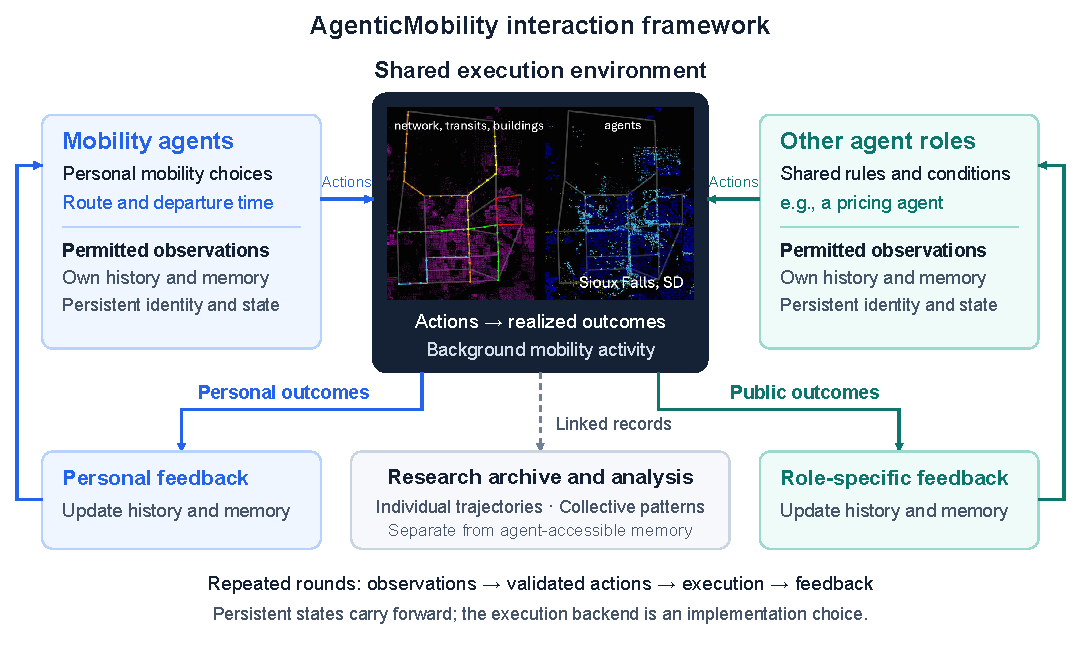
\includegraphics[width=1\textwidth, trim=0cm 1cm 0cm 1cm, clip]{pic/agenticmobility_framework_siouxfalls.pdf}
    \caption{AgenticMobility interaction framework.
Agents submit actions to a shared execution environment
and receive feedback according to their roles.
Persistent states carry experience across rounds, while
a separate research archive links decisions, execution,
and outcomes for analysis.}
    \label{fig:framework}
\end{figure}


\subsection{Roles, Observations, and Persistent State}
\label{sec:roles-state}

Each agent has a role, fixed attributes, an admissible action space, and a persistent state. The role determines which decisions the agent can make and which information it receives. Mobility agents act on personal activity requirements and experiences; other roles can use aggregate observations to change shared rules or costs. Roles may have different decision schedules while operating in the same environment.

Observations are assembled according to explicit access rules. They can include static descriptions, currently available announcements, and outcomes of earlier actions. Outcomes of an action become available only after its execution. Private records remain associated with their permitted roles, while shared announcements and public summaries follow the study's visibility rules.

To carry experience across rounds, each agent retains recent
observed outcomes and a bounded summary of earlier experience.
Observed outcomes and generated summaries are stored
separately, distinguishing environmental records from the
agent's interpretations. Facts retain observed outcomes; bounded summaries carry selected experiences and interpretations into later rounds. Each agent maintains its own state. The research archive preserves the more complete interaction record for inspection without providing unrestricted retrieval to agents. This separation makes memory availability and information access explicit experimental choices.


\subsection{Action and Execution Interfaces}
\label{sec:actions}

An action is a structured request with an agent identifier, a decision time, and role-specific fields. The action interface defines valid values, units, timing, and scope. A mobility action can select a route or departure time; another role can change a shared rule or cost. Validation checks whether the request satisfies the configured constraints before it reaches the execution layer. Generated explanations are retained separately from the executable fields.

An execution adapter translates accepted requests into operations supported by the selected backend. The environment executes them jointly with background activity and resource constraints, then returns identifiable outcome records. The adapter must preserve action scope and timing and expose the information needed to check application, completion, and realized outcomes. A valid action does not guarantee the intended outcome:
shared constraints and other agents' activities can delay
execution or prevent completion. Selected actions and
realized outcomes are therefore recorded separately.

These requirements define the contract between the platform and its execution backend. Supporting another backend requires an adapter and checks of its action and observation semantics. The interface specifies what must be connected; the backend determines the environmental dynamics. Section~\ref{sec:reproducibility} describes the realization evaluated in this paper.

\subsection{Interaction Timing, Feedback, and Traceability}

Roles act according to their decision schedules within each
round. When one role changes shared conditions before another
decides, the coordination protocol specifies whether the
change is visible to the later decision-maker.
Figure~\ref{fig:interaction_timing} summarizes the sequence
from condition updates and action selection to execution,
feedback, and state updates.

Agents interact by changing the conditions encountered by
others or the aggregate outcomes observed by another role.
The current framework supports these interactions through
the shared environment, without requiring direct messages
between agents. Role-specific feedback updates persistent
states, carrying experience into subsequent rounds.

For each decision, the archive links the supplied input,
generated action, validation result, applied action,
realized outcome, and subsequent state update.
These records allow researchers to distinguish changes in
agent choices from discrepancies in action application
or feedback timing. Active policies and failure handling
are also recorded. Appendices~\ref{app:concrete-protocol} and~\ref{app:implementation} specify the implemented
daily protocol and the conditions for retrying, retaining
a prior state, or stopping execution.

\begin{figure}[!htbp]
    \centering
    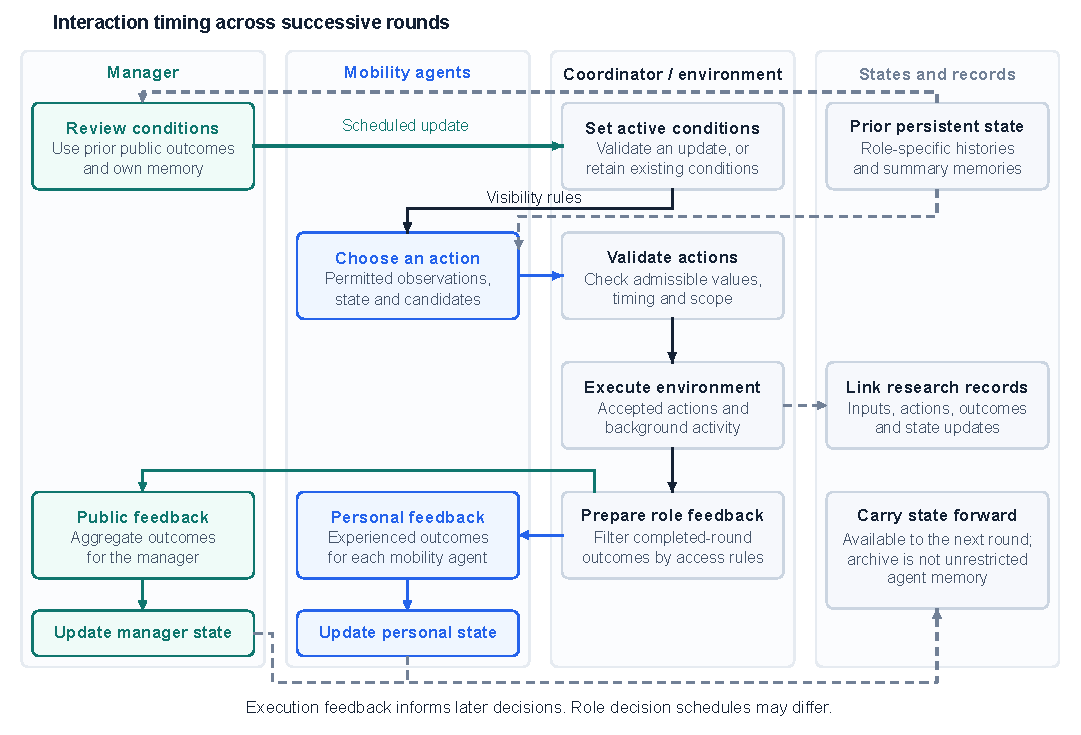
\includegraphics[width=\textwidth, trim=0cm 0cm 0cm 0cm, clip]
        {pic/interaction_timing.pdf}
    \caption{Interaction timing and state updates across
    successive rounds. Solid arrows indicate action and
    feedback flows; dashed arrows indicate state transfer
    or research-record linkage. Execution feedback informs
    subsequent decisions, while the research archive remains
    separate from agent-accessible memory.}
    \label{fig:interaction_timing}
\end{figure}




\section{Implementation and Reproducibility}
\label{sec:reproducibility}

The current implementation realizes the framework with MATSim as the execution backend \cite{horni2016matsim}. LLM traveler agents choose routes and departure times for fixed target trips; an LLM manager periodically sets link charges. Background trips retain the backend's behavioral mechanisms and full-day activity chains. The adapter applies validated choices and policies and extracts individual and aggregate feedback. The demonstration evaluates execution consistency in this
implementation; other execution backends have not been
evaluated.Appendix~\ref{app:concrete-protocol} specifies the implemented action, information, and daily-update protocols.

\subsection{Code, Dependencies, and Scenario}

The project entry point is \url{https://github.com/Agentic-City-Research/Agentic-Mobility}. The supplied distribution documentation specifies JDK~25, the Maven Wrapper, and MATSim~2026.0. The experiment launcher is \texttt{org.matsim.agentic.MorningExperiment}; despite its historical name, it runs full-day activity chains. Code is distributed under GPL-2.0, with separate notices for third-party components. The README links installation, method, experiment, and scenario guides.

The synthetic scenario derives from the enriched Sioux Falls study \cite{chakirov2014sioux} and Ben-Dor's version-3 car-traffic dataset \cite{ben-dorPopulationDownscalingMultiagent2021}, available under CC BY~4.0. The distribution includes the network, facilities, and population inputs referenced by \path{scenarios/SiouxFalls-public/config.xml}. Its original-demand population is restored by removing verified duplicates from the doubled-population source. The scenario guide and \path{THIRD_PARTY.md} document these transformations and input hashes; distributed-file hashes do not constitute a fresh byte-for-byte comparison with upstream downloads. These are synthetic research inputs, not observed resident trajectories.


\subsection{Execution Entry Points}

The documented installation check uses 100 simulated people, two days, and no LLM calls. From a Bash shell with Git and JDK~25 available:
\begin{quote}\footnotesize
\begin{verbatim}
git clone https://github.com/Agentic-City-Research/Agentic-Mobility.git
cd Agentic-Mobility
sh ./mvnw -B clean package
java -Xmx4g -cp matsim-example-project-0.0.1-SNAPSHOT.jar \
  org.matsim.agentic.MorningExperiment \
  --config scenarios/SiouxFalls-public/config.xml \
  --mode hybrid --policy mnl --llm-agents 0 \
  --demand 100 --sample-persons 100 --days 2 \
  --population-seed 4711 --seed 4711 --output output/quickstart
\end{verbatim}
\end{quote}
Completion is indicated by \texttt{complete=true} and \texttt{daysCompleted=2} in \path{morning/status.json} under the output directory reported by the application. Existing directories cause a numbered alternative to be selected. The Windows build command is \verb|.\mvnw.cmd -B clean package|; the README supplies PowerShell launch syntax. This small diagnostic checks installation and environmental execution; its sampling option does not scale road capacity.

Enabling LLM roles additionally requires a Chat Completions-compatible service, configured through \texttt{AGENTIC\_BASE\_URL}, \texttt{AGENTIC\_MODEL}, and \texttt{AGENTIC\_API\_KEY}, together with the role settings described in the experiment guide. Appendix~\ref{app:decision-models} records the archived model and prompt settings. A role-enabled execution check should inspect accepted actions, returned experiences, and memory updates across successive rounds; these are distinct from the installation check above.

\subsection{Relation Between the Distribution and Reported Runs}

The documentation package describes the completed 100-day, seed-268 runs. The package contains aggregate time series, run summaries,
and audit records corresponding to the appendix. The individual-case records support the execution example in Section~\ref{sec:validation}. These materials support inspection of recorded outputs.

Exact reruns additionally require the run-specific executable, input and candidate files, original prompts, final configuration, and model-service settings. 
The released records support inspection of the reported
outputs, but a traffic seed alone does not fix remote model responses. A pinned release-to-run mapping is therefore needed before claiming exact computational reproduction.
\section{Execution Validation and Illustrative Use}
\label{sec:validation}

We examine whether the implemented platform connects agent
decisions, environmental execution, and subsequent feedback as
specified. Execution checks and an individual trace assess
these connections, while aggregate outputs illustrate how the
platform supports studies of individual adjustment and
collective dynamics.


\subsection{Demonstration Setup}
\label{sec:demonstration-setup}

The demonstration uses an enriched Sioux Falls scenario with
16,822 simulated people and 11,793 fixed target trips. Full-day
activity chains and background mobility remain active in all
configurations. Table~\ref{tab:conditions} summarizes five
configurations that vary the target-trip decision mechanism
and the presence of an LLM manager. All use MATSim for
environmental execution.

\begin{table}[htbp]
    \centering
    \small
    \caption{Demonstration configurations. Trips outside the
    controlled target set retain MATSim behavioral mechanisms.
    MNL and LLM traveler agents select target actions from
    fixed route and departure-time sets.}
    \label{tab:conditions}
    \renewcommand{\arraystretch}{1.15}
    \begin{tabularx}{\linewidth}{
        @{}
        >{\raggedright\arraybackslash}p{0.29\linewidth}
        >{\raggedright\arraybackslash}X
        >{\raggedright\arraybackslash}p{0.20\linewidth}
        @{}
    }
        \toprule
        Configuration & Target-trip decisions & manager \\
        \midrule
        MATSim
        & MATSim plan selection and replanning
        & Disabled \\

        MNL
        & Constrained joint route--departure choice
        & Disabled \\

        LLM Traveler
        & LLM route--departure choice
        & Disabled \\

        MATSim + Manager
        & MATSim plan selection and replanning
        & Enabled \\

        LLM Traveler + Manager
        & LLM route--departure choice
        & Enabled \\
        \bottomrule
    \end{tabularx}
\end{table}

Each configuration completed 100 simulated days with simulation
seed 268. The comparison contains one run per configuration;
successive days share persistent states and are not independent
replications. Some executable builds differ, and the MNL
coefficients are uncalibrated. The results therefore describe
the recorded configurations rather than isolate individual
mechanisms. Detailed settings and measurement definitions are
provided in the appendices.

Day indices in this section follow the zero-based logs,
from Day0 to Day99. Pricing review opportunities occur on
Days20, 50, and 80. Positive charging begins on Day20 in
MATSim + Manager and on Day50 in LLM Traveler + Manager.
The figure labels Native, Traveler, Manager, and Joint
correspond to MATSim, LLM Traveler, MATSim + Manager,
and LLM Traveler + Manager, respectively.


\subsection{Execution and Feedback Consistency}
\label{sec:validation-execution}

All five configurations completed 11,793 target trips and 33,644 car legs per day, with no stuck agents. Work-arrival records cover the same 11,332 targets. Table~\ref{tab:execution-audit} separates checks of the combined run from the sampled inspection of decision inputs.

\begin{table}[tbp]
\centering\small
\caption{Execution audit scope and results. Full-record checks concern LLM Traveler + Manager; the information-access check covers the inspected samples only. Action checks apply to finalized outputs after validation and repair.}
\label{tab:execution-audit}
\renewcommand{\arraystretch}{1.15}
\begin{tabularx}{\linewidth}{@{}>{\raggedright\arraybackslash}p{0.25\linewidth} >{\raggedright\arraybackslash}p{0.29\linewidth} >{\raggedright\arraybackslash}X@{}}
\toprule
Check & Coverage & Recorded result \\
\midrule
Action constraints and execution & 1,179,300 finalized target decisions & Valid route and departure choices; accepted actions linked to applied plans and completed routes \\
Personal state continuity & 100-day personal memory chains & Continuous chains; finalized summaries within the configured limit \\
Pricing decisions and state & 3 policy decisions; 100 daily memory updates & Valid policy decisions; all daily memory updates completed \\
Information access & 4,000 sampled input contexts & No current announcements disclosed to uninformed travelers; no network-wide traffic information disclosed \\
\bottomrule
\end{tabularx}
\end{table}

Output repair affected 0.206\% of finalized travel-decision records and 0.250\% of personal-memory records. One manager-memory response required JSON repair. These results describe accepted outputs after validation and retry. Selected and realized departure times are recorded separately because preceding activities can delay execution. Appendix~\ref{app:audit-cost} reports exact repair counts and inference workload.

The audits check structured actions, recorded execution, and state continuity. Generated explanations and memory content require separate semantic checks, as the following cases illustrate.


\subsection{A Recorded Interaction Trace}
\label{sec:interaction-trace}

Figure~\ref{fig:execution-trace} follows synthetic traveler \texttt{10010\_2} in LLM Traveler + Manager. On Day~60, the agent selected route \texttt{c1} and the earliest available departure after receiving recent outcomes that included a late arrival on Day~59. The applied action and completed route matched the choice; the resulting outcome entered the rolling personal history for subsequent decisions.

\begin{figure}[!htbp]
\centering\small
\fbox{\begin{minipage}{0.94\linewidth}
\textbf{Observation before the Day~60 decision.} Four candidate routes, nine departure options, a 09:00 arrival reference, personal outcomes from Days~57--59, and current toll announcements. Network-wide conditions are unavailable. The Day~59 trip arrived at 09:10:48.\par\smallskip
\centerline{$\downarrow$}
\textbf{Structured action.} Route \texttt{c1}, departing at 05:56:43: the earliest available option and 90 minutes before the original plan.\par\smallskip
\centerline{$\downarrow$}
\textbf{Execution and recorded outcome.} Applied and realized actions agree with the record; the completed route matches \texttt{c1}. Car time is 21.97 minutes, destination arrival is 06:33:36, and payment is zero. Door-to-door time is 36.88 minutes and uses different boundaries from car time.\par\smallskip
\centerline{$\downarrow$}
\textbf{Subsequent decision.} On Day~61, the traveler selects \texttt{c0} at 05:56:43. The Day~60 outcome is available in the rolling personal history.
\end{minipage}}
\caption{A recorded interaction trace connecting permitted observations, a structured action, realized execution, and a subsequent decision. The case illustrates traceability; route, departure time, and shared conditions vary together.}
\label{fig:execution-trace}
\end{figure}

The case was selected to illustrate an inspectable decision sequence. Both route and departure time changed between Days~59 and 60, alongside changing environmental conditions, so the trace does not isolate their individual effects. A separate checked case illustrates an explanation inconsistency: traveler \texttt{10042\_2} on Day~61 selected a departure time of 07:46:19 and departed at that
time, while its generated explanation stated 07:49:39.. The executable action remained consistent with its record. These cases demonstrate what the archive can reveal; they do not estimate the prevalence of explanation errors.
\FloatBarrier

\subsection{Illustrative Collective Dynamics}
\label{sec:illustrative-use}

\paragraph{Individual and system-level outcomes.}

The configuration with the lowest population-wide car time
differs from the one with the shortest target-trip time. LLM Traveler records the lowest mean daily car time per
person, 19.90\% below MATSim, whereas LLM Traveler + Manager
records the shortest mean target-trip time. Relative to
LLM Traveler, the combined configuration has 6.63\% lower
target-trip time but 14.62\% higher mean daily car time
per person. Differences already exist before positive charging,
preventing attribution of this contrast to the manager
alone.

Figure~\ref{fig:outcomes} shows these trajectories across
different evaluation scopes. Mean daily car time per person
includes all car legs and waiting before network entry,
with total duration divided by the fixed population of
16,822 simulated people. Mean target-trip car time covers
the 11,793 controlled trips, while the work late-arrival
rate uses the fixed denominator of 11,332 work targets.
Together, these measures relate outcomes for controlled
trips to those across the full simulated population.

\begin{figure}[!htbp]
    \centering
    \includegraphics[
            width=\linewidth,
        trim= 0cm 0cm 0cm 0cm, clip
    ]{section/pic/outcomes.pdf}
    \caption{Individual and system-level mobility outcomes
across five configurations:
(a) mean daily car time per person (min/person);
(b) mean target-trip car time (min/trip); and
(c) work-target late-arrival rate (\%).
The denominators are 16,822 simulated people,
11,793 controlled trips, and 11,332 work targets,
respectively. Panel (a) includes all car legs and waiting
before network entry. Thin lines show daily values and
thick lines show trailing seven-day means.
Days~20 and 50 mark positive charging in Manager and Joint,
respectively; Day~90 marks the MATSim innovation cutoff.
Each configuration has one seed-268 run.}
    \label{fig:outcomes}
\end{figure}

\paragraph{Individual adjustment and aggregate patterns.}

The two LLM traveler configurations show relatively
persistent route choices alongside more frequent
departure-time adjustments. Across the 99 adjacent-day
transitions, LLM Traveler and the combined configuration change
routes in 3.08\% and 2.19\% of target decisions, respectively,
while changing departure times in 29.45\% and 28.04\%.
These overall rates include 2,780 targets with only one candidate
route. Among the 9,013 targets with multiple routes, the
corresponding route-switching rates are 4.03\% and 2.86\%.

\begin{figure}[htbp]
    \centering
    \includegraphics[
            width=\linewidth,
        trim= 0cm 0cm 0cm 0cm,
        clip
    ]{section/pic/behavior.pdf}
    \caption{Individual choice changes and aggregate route-flow
    turnover. (a) Population-wide route-switching rates across
    five configurations, shown on a logarithmic scale.
    (b) Departure-time adjustment rates for Traveler and Joint.
    (c) Individual route switching and net turnover of
    OD-specific route counts. Rates use all 11,793 targets
    over 99 adjacent-day transitions. Thin lines show daily
    values and thick lines show trailing seven-day means.
    Day50 marks Joint charging and Day90 marks the MATSim
    innovation cutoff.}
    \label{fig:behavior}
\end{figure}

Figure~\ref{fig:behavior} places individual changes alongside
aggregate route-flow turnover. Offsetting switches can leave
aggregate route counts relatively stable, making individual
adjustment and collective redistribution distinct measurements.
The decline in MATSim route switching near Day90 also reflects
the configured cutoff for route and activity-time innovation;
it cannot be interpreted solely as behavioral stabilization.

LLM Traveler and the combined configuration select departures
an average of 34.96 and 39.65 minutes earlier than the original
plans. Their time outcomes therefore need to be interpreted
together with schedule changes and the available action space.
These observations identify measurable dimensions of
agent-system dynamics without establishing learned habits,
coordination, or welfare improvements. Subsequent studies can
vary information, memory, and role interactions while retaining
the same execution and recording interfaces.

\FloatBarrier

\section{Scope and Research Directions}
\label{sec:scope}

AgenticMobility provides interfaces for studying how roles, information access, and retained experience shape repeated mobility interactions. The execution checks establish an operational basis for such studies, while the illustrative trajectories identify questions for independent replication, behavioral validation, and extensions of the framework.

\paragraph{Independent replication and controlled comparisons.}
The configuration and build differences in Section~\ref{sec:validation} motivate repeated runs under a common implementation with documented simulation and model-generation settings. Independent runs are needed to distinguish between-run
variability from day-to-day changes within a single run. To examine a particular mechanism, future experiments can branch from a common recorded state and vary announcement access, memory availability, or a role's actions. Implementing and checking state restoration would be part of that design. Outcomes should include effects on agents outside the directly modified group, since they share the execution environment.

\paragraph{Behavioral calibration and semantic validation.}
Route persistence and earlier departure in Section~\ref{sec:illustrative-use} motivate tests of sensitivity to candidate actions, schedule assumptions, and retained experience. Observed choices and mobility records can guide calibration, with evaluation on held-out people, periods, or scenarios. Individual choices and aggregate flows require separate checks. The explanation inconsistency in Section~\ref{sec:validation} also motivates systematic inspection of summaries and reasons against their supplied inputs and recorded actions. Such inspection would complement execution audits by assessing the content retained across rounds.

\paragraph{Roles, information, and execution backends.}
Additional roles, such as service providers or resource-allocation agents, require explicit action spaces, observation permissions, and consequences for other agents. Alternative memory and information designs can be studied through the same recording interfaces. Supporting another execution backend requires an adapter and validation of action application, timing, measurement boundaries, and state continuity before comparing dynamics. Extensions to other urban functions would additionally require shared resource and state definitions across systems. Versioned implementations and accessible run-specific artifacts can support this progression from the current mobility realization.

\section{Conclusion}
\label{sec:conclusion}

AgenticMobility provides an open-source framework for repeated
interactions among mobility agents with different roles.
It connects role-specific observations, actions, and persistent
states to a shared execution environment through explicit
interfaces. The current implementation demonstrates this
process through LLM traveler agents and an LLM manager over five
100-day configurations. The platform provides an experimental basis for examining
how information, retained experience, and role interactions
shape individual choices and collective mobility dynamics.


% Bibliography
\clearpage
\bibliographystyle{unsrtnat}
\bibliography{references}

\clearpage
% Appendices
\appendix
\section{Implemented Mobility Protocol}
\label{app:concrete-protocol}

The following protocol instantiates the framework for the reported experiments. Its fixed target trips, daily rounds, route--departure actions, and link charges are implementation choices, rather than requirements on every future backend or study.

\subsection{Roles, Information, and Persistent State}
\label{sec:roles-state-implementation}

The road network is a directed graph $G=(V,E)$. Each simulated day $d=1,\ldots,D$ comprises full-day traffic execution and feedback. Agent identities, fixed attributes, experiences, summary memories, and active policies persist across days; vehicle movements are simulated anew.

LLM travelers control a fixed set of target trips, choosing routes and planned departure times. Target origins, destinations, modes, and candidate sets remain fixed. Their other trips and all trips by background travelers follow MATSim behavioral mechanisms, preserving full-day activity chains and replanning. An LLM pricing agent sets link charges; the archived implementation refers to this role as the manager. The roles interact through policies and shared traffic conditions, without direct exchanges of private information.

A traveler receives a synthetic profile, schedule references, candidate actions, static route information, recent personal outcomes, and a summary memory. Access to current toll announcements is fixed by person: informed travelers receive announcements relevant to their candidates; uninformed travelers learn from their own payments without observing the current policy. Past payments need not reflect current charges. Neither group receives network-wide real-time traffic information or realized travel times for unchosen routes. The comparisons below concern information supplied to controlled target decisions and their outcomes. Non-target trips retain background decision mechanisms and the same person-level announcement visibility assignment.

The manager receives public network information, aggregate traffic outcomes, policy history, and its own memory, excluding private traveler profiles and trip records. For each role, recent factual observations and a bounded LLM summary constitute the accessible history. The summary is replaced using the previous memory and new feedback; older experiences remain explicitly available only if retained in that summary. Full research archives are inaccessible to agents and distinguish environmental facts from generated interpretations.

\subsection{Travel and Management Actions}
\label{sec:actions-implementation}

For controlled target trip $i$, the traveler selects
\begin{equation}
    a_{i,d}=(r_{i,d},\tau_{i,d})\in\mathcal{R}_i\times\mathcal{T}_i,
    \label{eq:joint-action}
\end{equation}
where $\mathcal{R}_i$ and $\mathcal{T}_i$ are fixed route and departure-time sets. Routes satisfy network constraints, and departure times respect activity and simulation boundaries. The time grid is anchored to the original plan, rather than the previous day's choice. The LLM returns an action and a brief reason. Validity does not guarantee timely arrival or completion: preceding activities and trips can cause realized departure $\hat{\tau}_{i,d}$ to differ from selected departure $\tau_{i,d}$.

The manager periodically issues a complete policy assigning finite, nonnegative charges to eligible directed links. Unlisted links are free. The protocol limits the number of rules but imposes no preset price levels, upper price bound, or adjustment increment. If $p_d(e)$ is the charge per eligible entry to link $e$, target trip $i$ pays
\begin{equation}
    C_{i,d}=\sum_{n=1}^{N_{i,d}}p_d(e_{i,d,n}),
    \label{eq:realized-payment}
\end{equation}
where $e_{i,d,n}$ is the link entered at event $n$. Repeated entries incur repeated charges, and payments already incurred remain recorded for incomplete trips. Charges are constant within a day. For the same completed route and entry counts, changing departure time affects congestion and schedule outcomes but not the direct toll.

A valid policy replaces its predecessor; an empty policy removes all charges, and no update leaves the policy unchanged. The manager's task is to reduce full-day delay measured from completed link traversals. This measure differs from complete trip travel time, so evaluation also tracks completion, trip outcomes, and payments.

\subsection{Daily Execution and Feedback}
\label{sec:daily-cycle-implementation}

Each day follows a fixed sequence. First, the manager updates the policy when scheduled, using information available through day $d-1$. Travelers then choose actions from their permitted inputs. The simulator performs MATSim replanning, writes validated target actions into the plans, and executes all trips under the active policy. Individual outcomes and aggregate traffic summaries are returned to the respective roles, which update their memories for subsequent days. Travelers choose daily; the manager updates its memory daily and its policy periodically. The initial toll-free observation period also updates agent state.

Records distinguish selected actions, plan modifications, and realized execution, linking each to the relevant input, feedback, memory, and policy. These records support checks of action implementation and feedback timing. Failure handling and event bookkeeping are summarized in Appendix~\ref{app:implementation}.

\section{Demonstration Conditions}
\label{app:demonstration}
\label{sec:experimental-design}
\label{sec:scenario-conditions}

Table~\ref{tab:conditions} identifies the five recorded configurations. All use MATSim for traffic execution. MATSim agents select and replan activities and routes; constrained MNL and LLM travelers choose target actions within fixed candidate sets. Background trips retain MATSim mechanisms. The full set uses simulation seed 268 and paper days 1--100 (log Days~0--99). The archive labels \texttt{Native}, \texttt{Traveler}, \texttt{Manager}, and \texttt{Joint} correspond to MATSim, LLM Traveler, MATSim + Pricing, and LLM Traveler + Pricing, respectively. Population and information assignments use seed 6021; the fixed target cohort spans 2,877 OD pairs.



Management update opportunities occur on paper days 21, 51, and 81 after a 20-day toll-free period. MATSim + Pricing begins positive charging on day 21; LLM Traveler + Pricing retains zero charges until day 51, then charges links \texttt{43\_3} and \texttt{43\_4} at 1.5 scenario units per entry and retains these charges on day 81. The combined configuration assigns 5,897 travelers to current toll announcements and 5,896 to no current announcements, with personal feedback available to both groups.

Input checks cover network, population, facilities, capacities, target identities, and background settings. Candidate-based configurations share fixed route and departure options; MATSim agents are not restricted to those options. Matching inputs does not remove differences in executable builds, preference representations, or remote model responses. The MNL baseline uses uncalibrated homogeneous coefficients. Definitions and settings appear in the following appendices.
\FloatBarrier

% Technical appendix fragment. Insert after \appendix; do not add a document class.
% Packages: amsmath, array, booktabs, tabularx, placeins, hyperref.
% Sources: completed100 analysis reports and archived manifest_snapshots.json.
% Prompt descriptions below are summaries, not reconstructed original prompts.

\section{Scenario, Candidate Actions, and Configuration}
\label{app:configuration}

\subsection{Population and Target Selection}

The input scenario contains 84,110 people. Sampling sorts person identifiers, shuffles them with Java Random using seed 6021, and retains a fixed 20\% subset with all its plans, yielding 16,822 simulated travelers. Network flow and storage capacity factors are 0.2 and $0.2^{0.75}\approx0.2991$, respectively \cite{mersiniScalingMATSimTraffic2026,ben-dorPopulationDownscalingMultiagent2021}. Population sampling, synthetic profiles, information groups, and controlled-roster selection use seed 6021; the main simulation seed is 268.

Targets are selected from original plans using destination-activity start times in $[0,32400)$ seconds, corresponding to starts before 09:00. Selection covers all activity purposes and requires one car leg per target trip; it imposes no departure-window filter. Missing or invalid planned arrival times are excluded rather than imputed. The selected cohort contains 11,793 trips by 11,793 people across 2,877 OD pairs. Membership remains fixed throughout the experiment. The remaining 5,029 people and non-target trips of controlled people retain MATSim decision mechanisms. Work-arrival evaluation uses the fixed subset of 11,332 targets with work deadlines. The 09:00 selection threshold does not substitute for each trip's deadline.

\subsection{Fixed Candidate Sets}

Runs reuse the same precomputed BFS-LE candidate file \cite{rieser2013route}, validating topology, costs, overlap, and the shortest-route candidate without regenerating or reordering alternatives. The archived settings specify up to four candidates per OD pair and maximum pairwise overlap 0.85. For free-flow time, an alternative passes the detour check if its ratio to the reference is at most 2.5 or its excess time is at most 300 seconds. The analogous distance limits are 2.5 and 2,000 meters; both time and distance checks must pass. The exact overlap implementation and original candidate-file hash belong to the reproducibility archive.

Departure candidates span $-5400$ to $+1800$ seconds relative to the original planned departure, at 900-second intervals. Options are clipped against the original origin-activity start, day zero, and the exclusive simulation end; the original departure is retained. The arrival deadline is not a hard feasibility filter. Subsequent choices do not shift the original time anchor. Of the targets, 2,780 have one route and 9,013 have multiple routes; the former cannot contribute route switches within the fixed candidate space.

\begin{table}[htbp]
\centering\small
\caption{Principal archived settings for the 100-day experiment. Strategy weights are configuration weights, not probabilities inferred from their sum.}
\label{tab:configuration}
\renewcommand{\arraystretch}{1.15}
\begin{tabularx}{\linewidth}{@{}>{\raggedright\arraybackslash}p{0.35\linewidth}X@{}}
\toprule
Setting & Value \\
\midrule
MATSim version & 2026.0 \\
Population / simulation seeds & 6021 / 268 \\
Initial strategy weights & \texttt{ChangeExpBeta}: 0.7; \texttt{ReRoute}: 0.1; \texttt{TimeAllocationMutator}: 0.1 \\
Innovation cutoff & Log Day90, equivalent to paper day 91; existing-plan selection continues \\
Simulation interval for charging & $[0,108000)$ seconds \\
Manager opportunities & Paper days 21, 51, and 81 \\
Toll action limits & At most 40 distinct car links; finite nonnegative charge per entry; no preset price cap or increment \\
Recent personal observations & Up to three preceding days \\
Personal summary limit & 500 characters \\
Manager summary limit & 1,000 English words; target length 400--600 words, with no enforced minimum \\
Information groups & 5,897 informed and 5,896 uninformed; fixed person-level assignment \\
\bottomrule
\end{tabularx}
\end{table}

The effective innovation cutoff is established from the run logs and final configuration, rather than inferred solely from the initial strategy entries. Both background replanning and MATSim-agent target decisions are affected; LLM and MNL target choices continue under their respective decision mechanisms.

\section{Implementation, Information, and Execution Protocol}
\label{app:implementation}

This appendix describes how the current implementation
coordinates agent decisions, environmental execution,
and persistent states. It supplements the interaction
framework with implementation-specific information rules,
memory updates, output validation, and event bookkeeping.

\subsection{Implementation Components and Data Flows}
\label{app:implementation-components}

Figure~\ref{fig:implementation_dataflow} summarizes the
logical components of the current implementation.
The coordinator constructs role-specific inputs, schedules
decision and memory tasks, and validates generated outputs.
The execution adapter applies accepted choices and policies
in MATSim and extracts the outcomes needed for personal
and public feedback.

Agent-accessible histories and summaries support subsequent
decisions, while the research archive preserves linked
records for inspection. These components represent logical
responsibilities rather than separate deployed services.
The implementation distinguishes generated requests,
accepted actions, and realized outcomes throughout this
process.

\begin{figure}[!tbp]
    \centering
    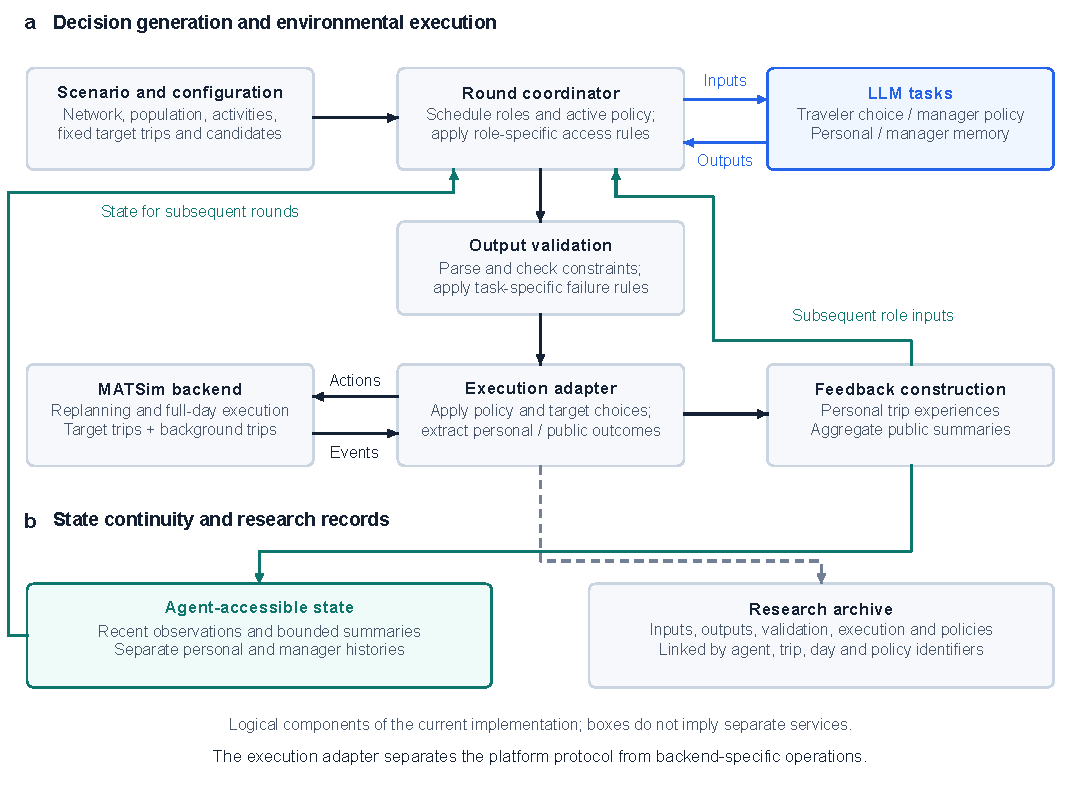
\includegraphics[width=\linewidth]
        {sections/pic/fig_implementation_dataflow.pdf}
    \caption{Logical components and data flows in the
    current implementation.
    (a) Role-specific inputs and generated outputs pass
    through coordination and validation before accepted
    actions are applied through the execution adapter.
    Returned events support personal and aggregate feedback.
    (b) Agent-accessible states support subsequent decisions,
    while a separate archive retains research records.
    Dashed arrows denote research-record linkage.}
    \label{fig:implementation_dataflow}
\end{figure}

\subsection{Information Access and Initialization}
\label{app:information-access}

Announcement visibility is assigned at person level:
all trips of a controlled person share the same visibility
assignment. The LLM selects actions only for the designated
target trip; other trips retain background routing and
time-adjustment mechanisms. For uninformed people, current
toll information remains unknown, although background
routing can retain personal link/time-bin observations.
People outside the treatment use the background
information mechanism.

Informed target decisions receive current toll estimates
for their candidate actions. Uninformed decisions receive
null current costs rather than zero costs. Both groups
receive static candidate information, recent personal
outcomes, and their own summaries, without network-wide
realized traffic conditions or outcomes for unchosen routes.
The LLM Traveler configuration explicitly communicates
that charging is disabled. In the combined configuration,
informed and uninformed inputs remain distinct even when
the active policy is empty.

Initial factual histories and self-written summaries are
empty. Synthetic profiles specify assumed preferences;
they do not represent observed past experiences.

The manager receives public network information, aggregate
reference-plan OD diagnostics, completion statistics,
aggregate link traffic, and its own policy and memory
histories. Private traveler profiles, memories, and
individual payments are excluded. The archived manager
projection retains the latest two executed policy-version
effects and pools older days, with aggregate recent/previous
statistics over windows of up to seven days. All-car links
remain represented in the public network, while detailed
traffic projection prioritizes high-delay or failed links
and currently or recently charged links. This projection
is distinct from the travelers' three-day personal window.

\subsection{Experience Retention and Memory Updates}
\label{app:memory-updates}

Figure~\ref{fig:memory_update} distinguishes recent factual
observations, generated summaries, and research records.
For each controlled traveler, completed-trip outcomes enter
a rolling personal history covering up to three preceding
days. A separate LLM task generates a replacement summary
from the previous memory and newly available feedback.
After validation, the new summary fully replaces the
previous one.

Personal histories and summaries remain associated with
the person and target trip and are not shared across agents.
No separate exact-payment history is available to the LLM
outside its bounded observations and summary. Once an
outcome leaves the recent-history window, its influence
through explicit historical context depends on what the
summary retains. The research archive preserves full
records for inspection but does not provide unrestricted
retrieval memory to agents.

Manager memory is updated after each completed day,
including toll-free days, independently of scheduled
policy decisions. Its inputs use public feedback and
the manager's own history. A memory update does not
change the active policy.

\begin{figure}[!tbp]
    \centering
    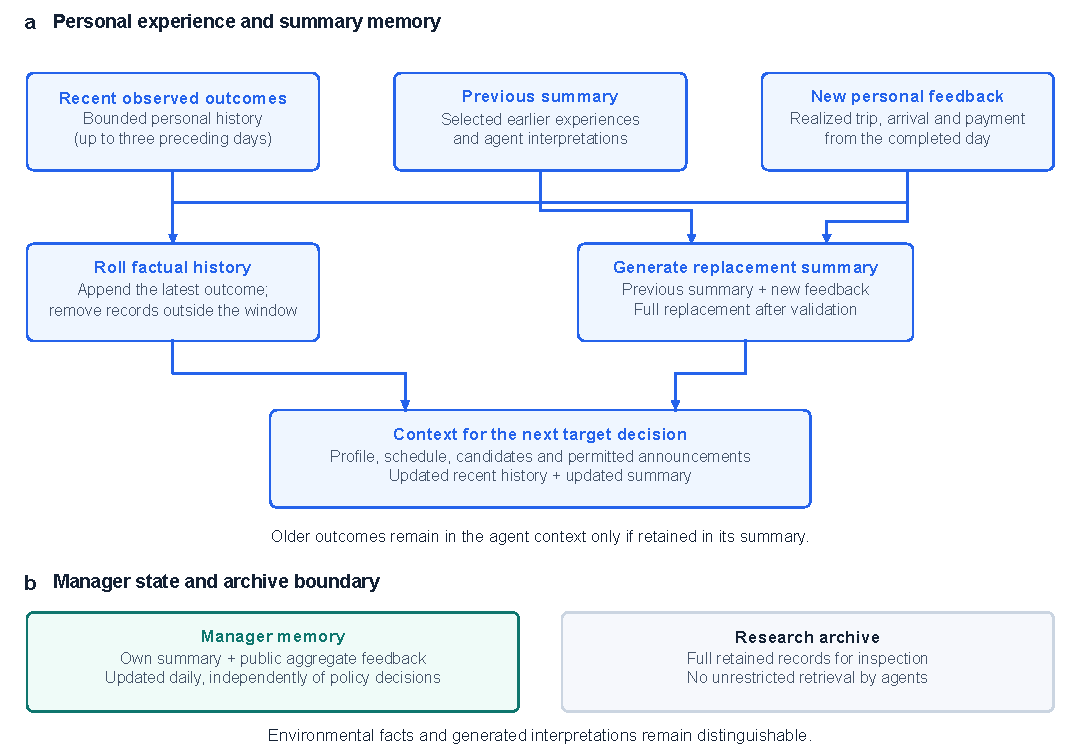
\includegraphics[width=\linewidth]
        {sections/pic/fig_memory_update.pdf}
    \caption{Experience retention and memory updates.
    (a) New personal feedback updates the rolling factual
    history and supplies a separate summary-generation task.
    The updated history and validated replacement summary
    enter subsequent target-decision contexts.
    (b) Manager memory is updated daily from public feedback,
    independently of policy decisions. Research archives
    remain separate from agent-accessible histories.}
    \label{fig:memory_update}
\end{figure}

\subsection{Output Validation and Failure Handling}
\label{app:output-validation}

Figure~\ref{fig:validation_failure} summarizes the validation
stages and task-specific failure rules. Traveler outputs
are checked for exact JSON, permitted route and departure
values, and configured character limits. Each task permits
at most three output attempts: the initial attempt and
up to two retries. Truncated responses are rejected without
salvaging partial JSON or inventing actions. Persistent
traveler-decision or personal-memory failure terminates
the experiment rather than silently substituting a stale
summary.

Failed or invalid manager-memory updates retain the
previous memory. The next successful update includes
the missing days. Manager-policy failures follow the
configured policy-failure protocol; detailed retry,
fallback, and transport-error handling must be interpreted
with the archived implementation. Output-repair counts
alone do not characterize these paths.

Structured-output validation does not establish semantic
accuracy. References to unavailable route identifiers
within summary text are logged diagnostically rather than
automatically rewritten. Semantic review was disabled in
the reported runs, so syntactic validity does not certify
the factual correctness of summaries or the faithfulness
of generated reasons. Late arrival and noncompletion are
environmental outcomes, not automatically output-format
failures.

\begin{figure}[!tbp]
    \centering
    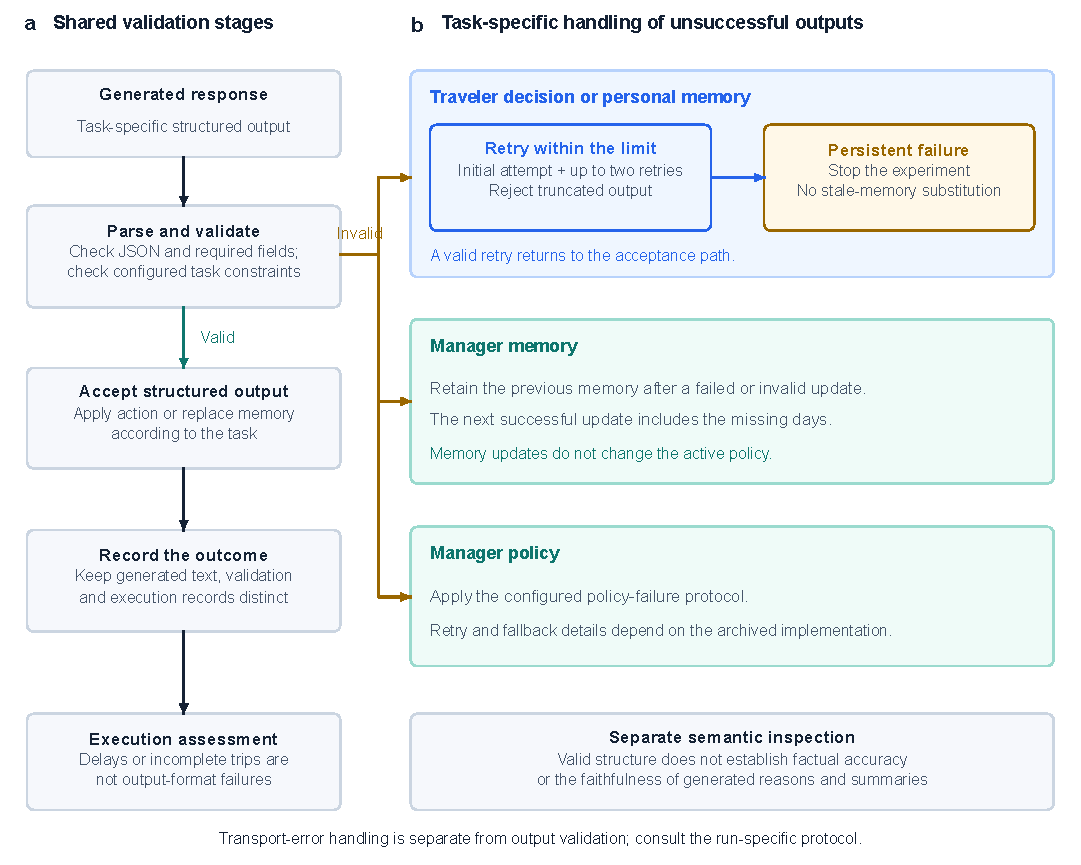
\includegraphics[width=\linewidth]
        {sections/pic/fig_validation_failure.pdf}
    \caption{Output validation and task-specific failure
    handling.
    (a) Structured outputs are checked before acceptance,
    with validation and execution recorded separately.
    (b) Persistent traveler-task failure stops the experiment;
    failed manager-memory updates retain the previous state.
    Manager-policy failures follow the configured protocol.
    Transport-error handling and semantic assessment remain
    separate from structured-output validation.}
    \label{fig:validation_failure}
\end{figure}

\subsection{Plan Execution and Billing}
\label{app:execution-billing}

Scheduled manager decisions precede environmental execution.
MATSim replanning is followed by writing validated route
and departure choices into the controlled target plans.
Other selected-plan activity ends are retained.
Original, selected, and realized departure times are
stored separately because preceding activities, queues,
and earlier trips can delay execution.

Tolls are charged on eligible car-link entries, including
the origin partial link under the archived billing
convention. Repeated traversals incur repeated charges,
while duplicate notifications of the same entry are
ignored. Charges apply over the half-open interval
$[0,108000)$ seconds and remain constant within a day.
Payments already incurred are retained if a trip
subsequently fails to complete. Candidate cost estimates
and actual payments are recorded separately.

A valid policy replaces the entire rule set, and an empty
policy removes all charges. Policy episodes are identified
by effective prices; a new version with unchanged prices
does not constitute a new price intervention.
Link-delay statistics use completed full-link traversals
and therefore have different event boundaries from toll
collection and trip-duration measurement.

\section{Measurement and Aggregation}
\label{app:measurement}

\paragraph{Choice changes and collective redistribution.}
Behavioral measures use selected actions, with realized departure times retained separately. Let $\mathcal{I}$ be the fixed cohort of $N=11{,}793$ targets and $\rho_{i,d}$ the complete ordered link sequence of the selected route. Population-wide rates are
\begin{equation}
 R_d=\frac{1}{N}\sum_{i\in\mathcal{I}}\mathbf{1}(\rho_{i,d}\ne\rho_{i,d-1}),
 \qquad
 A_d=\frac{1}{N}\sum_{i\in\mathcal{I}}\mathbf{1}(\tau_{i,d}\ne\tau_{i,d-1}),
 \label{eq:behavioral-adjustments}
\end{equation}
for paper days $d=2,\ldots,100$, corresponding to log transitions ending on Days~1--99. All targets have valid actions in these transitions. Candidate-based multi-route rates restrict both numerator and denominator to 9,013 targets; the remaining 2,780 cannot switch within their fixed route sets. MATSim agents are not restricted to those sets. A route is identified by its full link sequence, not its local candidate label. Aggregate route-flow turnover is $\sum_{o,r}|n_{o,r,d}-n_{o,r,d-1}|/(2N)$, where $n_{o,r,d}$ counts targets by OD pair $o$ and complete route $r$. Offsetting individual switches need not alter these counts.

Mean daily car time per person is calculated as
\[
\bar{T}^{\mathrm{car}}_d
=
\frac{60 T^{\mathrm{car}}_d}{16{,}822},
\]
where $T^{\mathrm{car}}_d$ is total daily car time in
person-hours. The normalized measure is reported in
minutes per person for each simulated day.

\paragraph{Time, schedule, and payment outcomes.}
Total daily car time sums car-departure-to-car-arrival durations across the population, including waiting before network entry. A complete total is undefined if a planned car trip is incomplete. Target-time distributions use completed target trips; completion and work-arrival measures retain their original cohort denominators. For 11,332 work targets, on-time completion, late completion, and noncompletion exhaust the cohort. All planned car trips completed in the reported runs.

Selected departure offsets are measured relative to original plans, and the earliest-option share counts selections of the earliest available candidate. Mean early arrival averages $\max(\mathrm{deadline}-\mathrm{arrival},0)$ over all work targets, including zeros. Mean daily P95 averages each day's target-time 95th percentile; individual savings compare each person's mean time over the common window. No monetary value is assigned to early arrival or departure inconvenience. Target payments and full-day personal payments use different trip scopes.

\paragraph{Aggregation and comparison windows.}
All five runs contribute paper days 1--100 (log Days~0--99). Outcome summaries average daily values over that window; relative changes are ratios of window means minus one, and lateness differences are percentage points. Choice-change rates average 99 adjacent-day transitions. Cutoff diagnostics treat log Day~90 separately and use Days~91--99 for the post-cutoff window. Plotted smoothing uses a trailing seven-day mean. Successive days and travelers within a shared run do not provide independent run-level replications.

Link-delay comparisons first aggregate original link records to full days to reconcile reporting intervals. Completed-link delay excludes waiting before network entry. Target/other-trip and waiting/post-entry decompositions each recover total car time and are alternative accounts of the same total.

\section{Execution Audit and Computational Workload}
\label{app:audit-cost}

Output repair was required for 2,433 finalized travel-decision records (0.206\%) and 2,943 personal-memory records (0.250\%). All personal memory chains were continuous, submitted memories remained within 500 characters, and no finalized travel decision was blank. The three management decisions were valid; one invalid management-memory JSON response was repaired through retry, with all 100 daily updates completed. These checks establish consistency of accepted outputs and state updates, without implying that every initial generation was valid or that generated reasons and memories were semantically correct.

\begin{table}[htbp]
\centering
\small
\caption{Recorded LLM inference workload over complete 100-day runs. Counts include retries and repairs across roles; tokens are service-reported totals. Zero LLM calls does not imply zero simulation cost.}
\label{tab:cost}
\begin{tabularx}{\linewidth}{@{}Xrr@{}}
\toprule
Condition & API calls & Tokens \\
\midrule
MATSim & 0 & 0 \\
MNL & 0 & 0 \\
LLM Traveler & 2,362,964 & 5,713,538,990 \\
MATSim + Pricing & 109 & 872,774 \\
LLM Traveler + Pricing & 2,364,090 & 5,451,720,152 \\
\bottomrule
\end{tabularx}
\end{table}

The combined run contains 1,181,736 traveler-decision calls, 1,182,250 personal-memory calls, three management-decision calls, and 101 management-memory calls. There are 1,179,300 finalized records for each personal task. The excess calls include repair and retry overhead and cannot be interpreted as hallucination counts. Logged tokens do not measure monetary cost, GPU energy, or end-to-end runtime. Semantic correctness of all memories and faithfulness of generated reasons have not been systematically established.

\section{Archived Demonstration Outputs}
\label{app:supplementary}

Tables~\ref{tab:validation-outcomes} and~\ref{tab:supp-switching} record selected outputs from one run per configuration at seed 268. They describe outputs of the recorded configurations and support the illustrative uses in Section~\ref{sec:illustrative-use}; their rankings are not estimates of general comparative effectiveness or robustness. Repeated days and person-days are dependent observations. Rounding limits display precision; it does not quantify uncertainty. Full-precision aggregate data are retained in the accompanying 100-day documentation package.

\begin{table}[htbp]
    \centering
    \small
    \caption{Archived output summaries over the common 100-day window (traffic seed 268). Entries are daily means, rounded for display; rankings apply only to these recorded runs. Total car time includes all car trips and waiting before network entry; work lateness uses the fixed denominator of 11,332 trips. These are summaries of one run per configuration, not independent-replication estimates.}
    \label{tab:validation-outcomes}
    \renewcommand{\arraystretch}{1.15}
    \begin{tabularx}{\linewidth}{@{}>{\raggedright\arraybackslash}X r r r@{}}
        \toprule
        Condition & \shortstack{Total car time\\(person-h/day)} & \shortstack{Target time\\(min/trip)} & \shortstack{Work lateness\\(\%)} \\
        \midrule
        MATSim & 12,431 & 29.3 & 20.0 \\
        MNL & 17,201 & 53.2 & 31.3 \\
        LLM Traveler & 9,958 & 17.4 & 5.6 \\
        MATSim + Pricing & 12,663 & 29.6 & 20.4 \\
        LLM Traveler + Pricing & 11,414 & 16.3 & 3.7 \\
        \bottomrule
    \end{tabularx}
\end{table}

\begin{table}[htbp]
\centering\small
\caption{Mean daily choice-change rates over 99 adjacent-day transitions. Overall rates use 11,793 targets; multi-route rates use 9,013 eligible targets. A dash denotes a candidate-space comparison that is not applicable. All entries are percentages.}
\label{tab:supp-switching}
\begin{tabularx}{\linewidth}{@{}Xrrr@{}}
\toprule
Condition & \shortstack{Overall\\route changes} & \shortstack{Multi-route\\changes} & \shortstack{Departure\\changes} \\
\midrule
MATSim & 5.26 & --- & 20.05 \\
MNL & 48.55 & 63.52 & 85.24 \\
LLM Traveler & 3.08 & 4.03 & 29.45 \\
MATSim + Pricing & 5.43 & --- & 20.28 \\
LLM Traveler + Pricing & 2.19 & 2.86 & 28.04 \\
\bottomrule
\end{tabularx}
\end{table}

A supplementary MATSim--pricing pair at seed 9261 is retained in the archive. It is not a replication of the five-condition experiment or the information-group comparison. Its presence does not change the single-run scope of the tables above.

\subsection{Run-Specific Reproduction Artifacts}
\label{app:archive-scope}

The analysis archive preserves effective configurations, input and executable hashes, candidate sets, accepted actions, attempts, experiences, policy histories, and memory updates. The distribution documentation supplies aggregate CSVs and audit summaries. A run-specific reproduction bundle must additionally identify the corresponding code revision or executable, original prompt templates, model-service settings, and input versions. Public access locations and the mapping from release artifacts to historical builds should accompany that bundle; the scope supported by the current documentation is described in Section~\ref{sec:reproducibility}.
% AUTHOR CHECK: Supply verified immutable release/run identifiers and accessible
% raw-artifact locations before claiming exact historical regeneration.
\FloatBarrier



\end{document}